\chapter{Doble propulsor. Segunda iteración}
Es momento de trabajar en serio, en esta ocasión no avanzaré al siguiente objetivo
si no se cumple primero el presente, para ello si lo requiero repetiré el proceso
de manera continua tratando de mejorar el trabajo previo.
\section{Requerimientos}
El objetivo es casi el mismo solo adicionamos una especificación.
\begin{itemize}
	\item Mover el robot hacia adelante.
	\item Utilizar un tren de propulsión de dos unidades.
\end{itemize}
\section{Análisis}
Nuevamente aprovechare el trabajo previo.
\begin{itemize}
	\item Rediseñar el circuito, adicionando el segundo propulsor.
	\item Rediseñar la base acomodando ambos propulsores.
	\item Rediseñar el programa para dos propulsores.
\end{itemize}
\section{Diseño}
Estamos a tiempo para implementar estos cambios, tienen un gran impacto, pero la
forma modular que adopte me facilita hacerlos sin mucha perdida de tiempo.  
\subsection{Arquitectura electrónica}
Agregar un nuevo motor es una trivialidad, basta con repetir el modulo del motor,
pero invirtiendo la polaridad, los motores estarán alineados
y para que el robot 
avance, un motor debe girar en sentido dextrógiro y el otro en levógiro.
El esquemático se muestra en la figura \ref{fig:Esquemático 2}.
\newschematic{img/esquematico2.pdf}{Esquemático 2}
\subsection{Arquitectura mecánica}
La actualización es sencilla, se reemplazan dos postes por dos motores y se 
retira el motor central, figura \ref{fig:Plano 2}.
\newdraw{img/plano2.pdf}{Plano 2}
\subsection{Arquitectura de software}
Robot requiere un modulo más abstracto que represente a los propulsores, 
propongo reemplazar Motor, por TrenDePotencia, el resto lo dejo igual por ahora,
figura \ref{fig:arquitecturaSoftware2}.
\begin{figure}[hbtp]
	\centering
	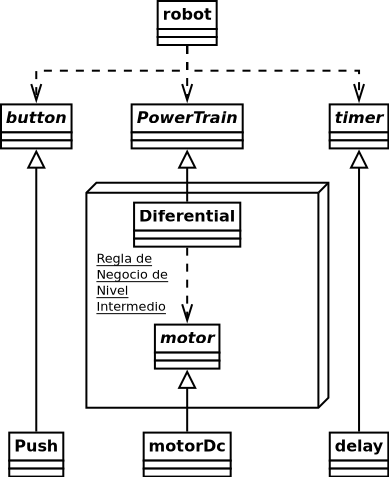
\includegraphics[scale=0.5]{img/arquitecturaSoftware2.png}
	\caption{Arquitectura de software 2}
	\label{fig:arquitecturaSoftware2}
\end{figure}

\section{Implementación}
\subsection{Implementación electrónica y mecánica}
No hay misterios cableamos y ensamblamos como indica el esquemático y plano.
\subsection{Implementación de software}
Esta parte requiere más cambios, creamos una nueva interfaz, llamada $PowerTrain$ 
que sustituye a $Motor$ pues esta última ya no nos sirve para esta etapa, 
implementamos un tren 
de potencia $Differential$, tan solo contiene dos referencias a dos motores, 
izquierdo y derecho y la respectivas implementaciones de las funciones virtuales
de $on$ y $off$. 
\begin{minted}[linenos]{C++}
#include "differential.h"
Differential::Differential(Motor * left, Motor * right)
	: rigth_{right}, left_{left}
{
}
void Differential::on(void)
{
	rigth_->on();
	left_->on();
}
void Differential::off(void)
{
	rigth_->off();
	left_->off();
}
\end{minted}
\subsubsection{Firmware}
La definición de firmware ha cambiado a lo largo del tiempo, hoy en día al firmware
se le identifica como el software que interactúa directamente con el hardware, en
términos de microcontroladores, el firmware es el software que interactúa directamente
con los registros. En nuestro caso tenemos firmware en la implementación de $MotorDc$ 
y en $Push$. 

Probablemente la forma correcta de escribir firmware es escribir menos firmware,
por naturaleza cambia junto con el hardware, es decir se vuelve obsoleto con los
cambios de hardware, prefiero aislarlo en una pequeña 
biblioteca y llamarlo desde $Motor$, en el diagrama de arquitectura 
figura \ref{fig:arquitecturaSoftware2}, no lo incluí pues la idea me surgió después
de diseñarlo,
pero no importa, pues la metodología me permite agregarlo posteriormente. La 
implementación de $Motor$ es:
\begin{minted}[linenos]{C++}
#include "motorDc.h"
#include "gpio.h"

MotorDc::MotorDc(short const pin) : pin_{pin}
{
	gpio_setDirection(pin_, OUTPUT);
}
void MotorDc::on(void)
{
	gpio_setLevel(pin_, HIGH);
}
void MotorDc::off(void)
{
	gpio_setLevel(pin_, LOW);
}
\end{minted}
Ahora $MotorDC$ ya no depende de los registros, la responsabilidad se pasa a dos
funciones $gpio\_setLevel$ y $gpio\_setDirection$, no es el objetivo atiborrar el 
presente documento de código, por lo que prefiero no presentar la implementación
de dichas funciones pues no forman parte del robot, son simples utilidades, el 
código completo está disponible en el repositorio.
\section{Pruebas}
Las expectativas son altas, pues la implementación y diseño fueron fáciles, 
increíblemente los resultados son un fracaso.
Ensamblado, actualizado y puesto en marcha obtengo las siguientes observaciones:
\begin{itemize}
	\item Avanza un par de milímetros y se detiene.
	\item En el aire las ruedas giran aveces.
\end{itemize}
Repitiendo varias veces el experimento me doy cuenta que cuando presiono el
botón el microcontrolador se reinicia.

En el pasado utilizamos solo un motor y funcionaba, sin embargo con dos motores 
la carga es demasiada para la fuente y por un instante la caída de tensión es
suficientemente alta como para que el microcontrolador se apague. 

Debo repetir todos los pasos y ajustar en donde considere necesario.
\section{Segunda iteración}
\subsection{Requerimientos y Análisis}
Sin cambios.
\subsection{Diseño}
\subsubsection{Diseño electrónico}
El problema es claramente eléctrico, la primera reacción es agregar un capacitor
grande
para suavizar el arranque del motor, sin embargo no me da buenas sensaciones, 
aveces funciona y en otras se sigue apagando, la solución temporal más sensata
es separar la fuente de los motores de la fuente del microcontrolador.

Por comodidad decido cambiar el tipo de pulsador por uno normalmente apagado,
los cambios se ven reflejados en el esquemático de la figura
\ref{fig:Esquemático 2.2}.
\newschematic{img/esquematico2.2.pdf}{Esquemático 2.2}
\subsubsection{Diseño mecánico}
Sin cambios.
\subsubsection{Diseño del programa}
Se agregan los cambios faltantes en la anterior iteración, figura 
\ref{fig:arquitecturaSoftware2.2}.
\begin{figure}[hbtp]
	\centering
	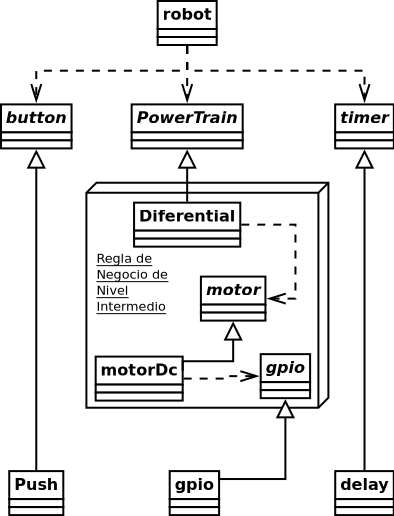
\includegraphics[scale=0.5]{img/arquitecturaSoftware2.2.png}
	\caption{Arquitectura de software 2.2}
	\label{fig:arquitecturaSoftware2.2}
\end{figure}
\subsection{Implementación}
El único cambio es agregar una batería como indica el esquemático, figura 
\ref{fig:Esquemático 2.2}.
\subsection{Pruebas}
¡Éxito!, el robot se mueve hacia adelante, observaciones:
\begin{itemize}
	\item Recorre alrededor de 1 metro.
	\item El movimiento es siempre con tendencia a la derecha.
	\item El microcontrolador ya no se apaga.
\end{itemize}
No requiero pruebas más exhaustivas para este requisito.
\section{Objetivos refinados}
\begin{itemize}
	\item Para el paciente.
		\begin{enumerate}
			\item Mover el robot de un punto A a B.
				\begin{itemize}
					\item \st{Mover hacia adelante}.
					\item Mover hacia atrás.
					\item Mover hacia adelante/atrás, en línea
						recta.
					\item Mover hacia adelante una x distancia.
					\item Mover hacia atrás una x distancia.
					\item Mover hacia adelante/atrás y girar hacia
						la derecha/izquierda.
					\item Girar x grados.
					\item Mover sobre una trayectoria curva.
				\end{itemize}
			\item Potencia suficiente para soportar la carga.
				\begin{itemize}
					\item \textbf{Fuente de controlador}.
					\item \textbf{Fuente de potencia}.
					\item Tamaño y materiales de la llanta.
					\item Motores con el tamaño y torque adecuado.
					\item Acoplamiento con la base.
				\end{itemize}
			\item Movimiento save.
				\begin{itemize}
					\item Control de la velocidad.
					\item Control de la aceleración.
					\item Control diferenciado de ambos motores.
					\item Generación y seguimiento de trayectorias.
				\end{itemize}
			\item Rotación libre.
				\begin{itemize}
					\item Basé rígida y pesada.
					\item Acoplamiento encima la base.
				\end{itemize}
		\end{enumerate}
	\item Para el médico.
		\begin{enumerate}
			\item Interfaz de trayectorias.
		\end{enumerate}
	\item Para el desarrollador.
		\begin{enumerate}
			\item Dominar un nuevo lenguaje de programación.
			\item Metodologías RUP y XP.
		\end{enumerate}
\end{itemize}
